\chapter{Extrapolation} \label{chap:outro}

\section{Next Steps in Extreme Wave Research}

\sidefigure{AI art generated by VQGAN + CLIP \citep{esser_taming_2021,radford_learning_2021}. Prompt: \emph{\enquote{a scientist looking at the ocean swell during sunset}}.}{
    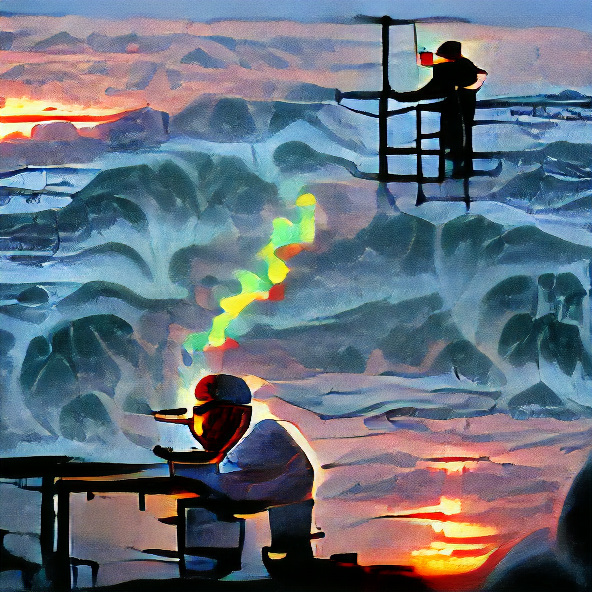
\includegraphics[width=.9\linewidth]{vqgan-images/vqgan-16.png}
}
%
The extreme wave research community is divided. Are rogue waves rare realizations in typical sea states or typical realizations in rare sea states? To make things worse, the term \enquote{rogue wave} is also used for extreme waves in other media such as optical fibers \citep[see \eg][]{dudley_rogue_2019}, with some overlapping creation mechanisms (like the modulational instability), but in general completely different characteristics. Discussions about rogue waves are therefore full of confusion and misunderstandings.

Our work has started to answer some of these questions: It looks like the vast majority of rogue waves in our data are rare realizations of typical sea states. This does not necessarily mean that nonlinear phenomena like solitons or breathers do not exist, just that they seem to not play a major role in \enquote{everyday} rogue wave generation. So what are the implications for the field? The following sections outline some --- in my opinion --- much needed further work.

\subsection{A More Meaningful Rogue Wave Definition}

When taking the rogue wave definition \eqref{eq:rogue} at face value, \emph{every} wave larger than the chosen threshold is a rogue wave, regardless of the underlying creation mechanism (and regardless of the absolute wave height). Yet, the rogue wave definition is only meaningful if these waves do not behave like the rest of the wave population\sidenote{As is implied by \enquote{rogue} or \enquote{freak}, as opposed to \enquote{unlikely wave}.}, so many authors choose to focus on examples where this is the case (whether or not they are represented in the real ocean).

We have shown that when we apply the rogue wave definition strictly, real-world rogue waves are well explained by bandwidth and directionality effects, plus some minor correction from weakly nonlinear dynamics. This may inform further research and lead to an improved understanding of the tail of the wave height distribution, which is valuable in itself, but it does not make a direct statement about the huge \emph{freaks} (like the Draupner wave) that people usually have in mind when talking about rogue waves\sidenote[-2.6]{Only if large rogue waves share the same generation mechanisms as small rogue waves, which is not obvious in the presence of nonlinearities.}.

A good definition is one that is helpful in the context where it is applied. If the goal is to study \emph{dangerous waves}, then other criteria that make waves dangerous should enter the definition, such as absolute height, steepness, or unexpectedness \citep{gemmrich_unexpected_2008}. If the goal is to study \emph{huge waves} or \emph{big storm waves} or \emph{highly nonlinear waves}, the definition should reflect that. A more sensible definition could help to unify the different view points on extreme waves, and bring engineers and physicists closer together.

\subsection{Firmer Anchoring in Observations}

In wave research, new theories are typically validated against simulations and wave plume experiments. Now that we have the tools for it (via datasets like FOWD and the analysis we developed), in-situ observations should play a bigger role in this process. This could help to shift the focus from conditional probabilities (if conditions X are met, Y will happen) to joint probabilities \citep[conditions X might never be met due to physical constraints, so Y is impossible; see also][]{mendes_physical_2021}.

There is much left to discover in FOWD and similar datasets, and we have only scratched the surface in terms of available data from many more providers. The field could profit tremendously from more rigorous empirical work, \eg by examining the role of currents on rogue wave formation.

\subsection{An Improved Operational Forecast}

Finally, an improved operational forecast for maximum expected wave heights is now within reach, for example one that includes the effects of crest-trough correlation and directionality on rogue wave probabilities. This should lead to clear improvements in terms of forecasting skill for typical rogue waves (something we plan to address in follow-up work).

Many accidents in the ocean involve rogue waves in sea states similar to the ones we have studied, and an improved forecast will allow for better planning of shipping routes to avoid the most dangerous conditions, or exploit conditions that are known to be safe.

\clearpage
\section{Next Steps in Machine Learning for Science}

\sidefigure{AI art generated by VQGAN + CLIP \citep{esser_taming_2021,radford_learning_2021}. Prompt: \emph{\enquote{cause and effect}}.}{
    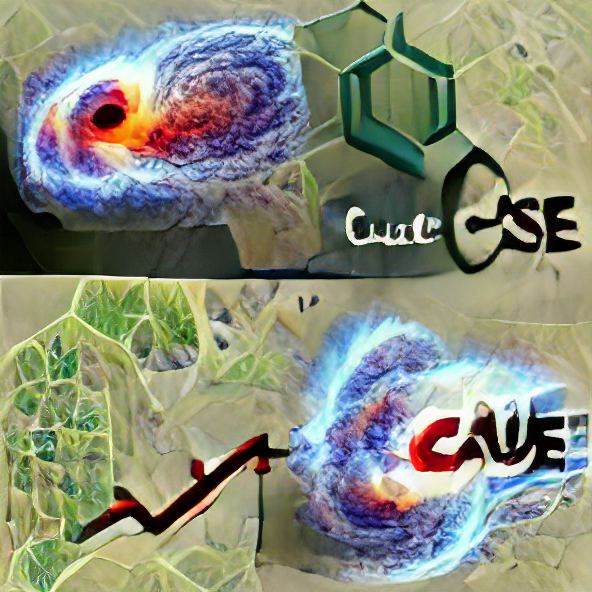
\includegraphics[width=.9\linewidth]{vqgan-images/vqgan-32.png}
}
%
In the study of physical systems, the combination of computation, data, machine learning, and causal reasoning is an extremely powerful one \citep{reichstein_deep_2019,lavin_simulation_2021}. Still, there is a long way to go before this approach becomes mainstream. The following sections outline some concrete steps towards this.

\subsection{More Methods Tailored to Physical Data}

Machine learning algorithms are usually not developed and evaluated with physical data in mind.
One example are classification problems on tabular data (like in this study), where tree-based methods like boosted trees \citep[\eg via XGBoost,][]{Chen:2016:XST:2939672.2939785} are typically found to perform best \citep{shwartz-ziv_tabular_2022}. However, most machine learning applications on tabular data are on \emph{human-centric} problems that have very different characteristics than physical problems, such as a vastly more complicated causal structure and discontinuous behavior.

As a consequence, methods other than the industry standard may be most appropriate on physical data. To address this, physical datasets should be accounted for during model evaluation by machine learning researchers to lead to methods that exploit \citebook{wigner_unreasonable_1960}, while making them more approachable for domain scientists.

\subsection{Tools for Uncertainty Estimation}

Reasoning under uncertainty is a staple in science, where answers that may be \enquote{good enough} in other domains (such as recommender systems) don't qualify, and where \enquote{I know that I don't know} is valuable information.

Most approaches to machine learning with uncertainties have long been prohibitively costly for large datasets like ours (\ie have non-linear scaling with the dataset size), such as Gaussian process regression or Bayesian methods based on Monte Carlo sampling. Modern techniques like sparse Gaussian processes \citep{leibfried_2020}, variational inference \citep{blei_variational_2017}, deep ensembles \citep{lakshminarayanan_simple_2017}, and stochastic weight averaging \citep{maddox_simple_2019,wilson_bayesian_2020} alleviate this, and represent a promising way towards integrating uncertainty information and machine learning. Still, more development is necessary for the widespread adoption of those or similar methods.

\subsection{Off-the-Shelf Causal Inference}

At its core, every scientific theory aims to describe a causal connection, so methods to identify and validate causality must be central to data-driven science.
But causality in arbitrary physical systems is often intractable, and the borders between association and causation are blurred in the presence of deterministic chaos and multi-scale interactions.

This calls for a formalization of causality in these systems on the one hand \citep[\eg as in][]{peters_causal_2020}, and methods for causal inference that are tailored to physical systems on the other hand (in a similar way as it has happened in medicine or econometrics). This may include techniques like invariant causal prediction \citep{peters_causal_2016} in connection with symbolic regression \citep{cranmer_discovering_2020}, which enables the identification of causally consistent machine learning models that can then be distilled into simple mathematical expressions for fully data-driven discovery of scientific theories.
